% ----------------------------------------------------------
\chapter{CLEAN - Collaborative Low-cost Environmental and Air-quality Network}\label{cap:clean-initiative}
% ----------------------------------------------------------
A iniciativa CLEAN consiste numa plataforma colaborativa para promover e facilitar o desenvolvimento de monitores de qualidade do ar de baixo custo, e o acesso remoto em tempo real a informações sobre a qualidade do ar. Possui quatro componentes principais: 

\begin{enumerate}
    \item Dispositivos de hardware
    \item Firmware reutilizável e bibliotecas de Programação Orientada a Objetos baseadas no framework Arduino para programação dos dispositivos de monitoramento
    \item A aplicação web \href{http://renovar.lcqar.ufsc.br/}{Renovar} para visualização (e acesso) remoto dos dados em tempo real
    \item Guias e documentação para reprodução do hardware e adesão à rede
\end{enumerate}

Todos os guias e documentação relativos ao desenvolvimento do hardware e firmware dos dispositivos até agora concebidos, as bibliotecas implementadas e as ferramentas de desenvolvimento estão abertas e disponíveis gratuitamente na \href{https://lcqar.ufsc.br/novo/index.php/documentacao-clean/}{página inicial de CLEAN}.

CLEAN permite a colaboração de outros grupos e indivíduos interessados no desenvolvimento de dispositivos de monitoramento de baixo custo e dados abertos para análises ambientais. A aplicação web Renovar fornece uma API que permite que diversos dispositivos de monitoramento de baixo custo enviem seus dados para um servidor remoto para visualização e armazenamento em tempo real e geolocalizados. Esses dados permanecem disponíveis abertamente para posterior processamento e análise. Dada a grande versatilidade dos sensores de baixo custo, muitas aplicações poderiam ser monitoradas a partir de diversos cenários, contribuindo para a disponibilidade de grandes volumes de dados. A continuação serão descritos os componentes principais da iniciativa CLEAN.

\section{Dispositivos de hardware desenvolvidos}

Dentro do contexto da iniciativa CLEAN foram desenvolvidos dispositivos para medição da qualidade do ar. Dois desses dispositivos foram protótipos para validação da ideia, concebidos para medições em locais fixos e medições móveis. Numa segunda etapa foram desenvolvidos dispositivos mais robustos com placas de circuito impresso e quadros elétricos para instalação em campo. A continuação serão descritos os equipamentos produzidos.

\subsection{Protótipos de monitores de qualidade do ar de baixo custo}

Foram concebidos dois protótipos de baixo custo para medição de poluentes atmosféricos \cite{Campo2020DEPLOYMENTRESULTS}, um para monitoramento fixo e outro para monitoramento móvel. O hardware de ambos os dispositivos, conforme mostrado na Figura \ref{fig:device-structure}, é composto por três blocos principais: 1) transporte de gás, 2) sensoriamento e 3) microcontrolador. O estágio de transporte de gás captura o ar ambiente nos sensores, que produzem um sinal analógico proporcional à concentração do gás. O microcontrolador, que é um Microchip ATMega2560 embarcado em uma plataforma Arduino Mega, captura as respostas dos sensores e as transforma em dados de concentração de gás. O hardware também obtém a hora e o local onde cada medição foi coletada. O microcontrolador armazena essas informações em um cartão micro SD e as transmite para um servidor web hospedado na Superintendência de Tecnologia da Informação e Comunicação da Universidade, rodando o aplicativo Renovar Web. Uma conexão Wi-Fi é estabelecida por um microcontrolador ESP8266 para transmissão de dados. Um relógio em tempo real e um módulo GPS fornecem informações de data, hora e geolocalização, respectivamente.

\begin{figure}
    \centering
    \caption{Estrutura principal dos dispositivos. a) Medidor de gases fixo, e b) medidor móvel}
    \includegraphics[width=1\linewidth]{chapters//2-CLEAN//Figuras/Estrutura geral protótipos.png}
    \label{fig:device-structure}
\end{figure}

A versão fixa dos dispositivos de monitoramento (Figura \ref{fig:device-structure}a) utiliza seis sensores eletroquímicos do fabricante de sensores Alphasense e quatro sensores eletroquímicos do fabricante SPEC Sensors. Para alimentação de energia do dispositivo utiliza-se uma fonte de 12VCC. Este dispositivo não incorpora módulo \textit{GPS} para geolocalização. A versão móvel (Figura \ref{fig:device-structure}b), por outro lado, utiliza apenas quatro sensores eletroquímicos do fabricante SPEC Sensors. O dispositivo é alimentado por um banco de energia de 5VCC através de uma conexão USB. A Figura 3 ilustra ambos protótipos na versão fixa e móvel. Mais detalhes sobre os dispositivos podem ser encontrados no Apêndice \ref{apendix: hw-prototypes}.

\begin{figure}
    \centering
    \caption{Ilustrações das versões (a) fixa e (b) móvel dos dispositivos de monitoramento}
    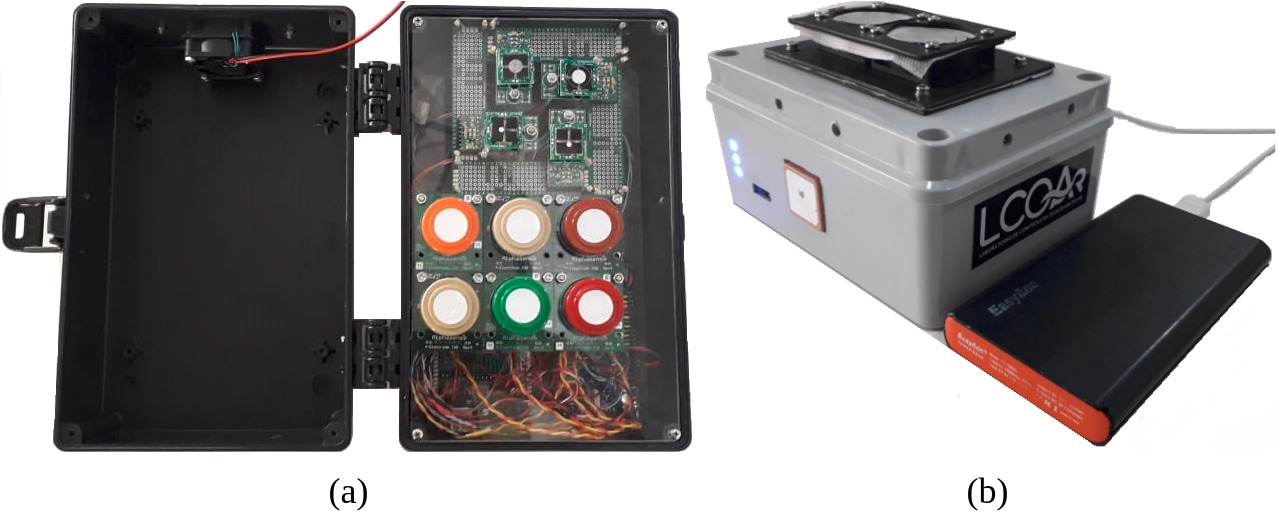
\includegraphics[width=1\linewidth]{chapters//2-CLEAN/Figuras/Monitoring Prototypes.jpg}
    \label{fig:monitoring-prototypes}
\end{figure}

\subsection{A placa CLEAN Arduino MEGA}

Com base nos resultados obtidos pelos protótipos e nas experiências alcançadas, foi desenvolvida uma versão mais compacta e atualizada para monitoramento fixo. Esta versão foi chamada de \textit{CLEAN Arduino Mega Board} por causa do microcontrolador Arduino Mega que ela usa como processador principal. A composição do hardware é muito semelhante à dos protótipos, mas os módulos foram montados em uma única \textit{PCB}. A Figura \ref{fig:clean-arduino-mega-board} ilustra o projeto da PCB e uma das placas fabricadas. A PCB foi criada no \textit{software} Eagle, e os arquivos do projeto estão disponíveis nos repositórios do LCQAr da UFSC.

\begin{figure}
    \centering
    \caption{A placa CLEAN Arduino Mega: (a) projeto PCB, (b) vista superior da placa, (c) vista inferior da placa.}
    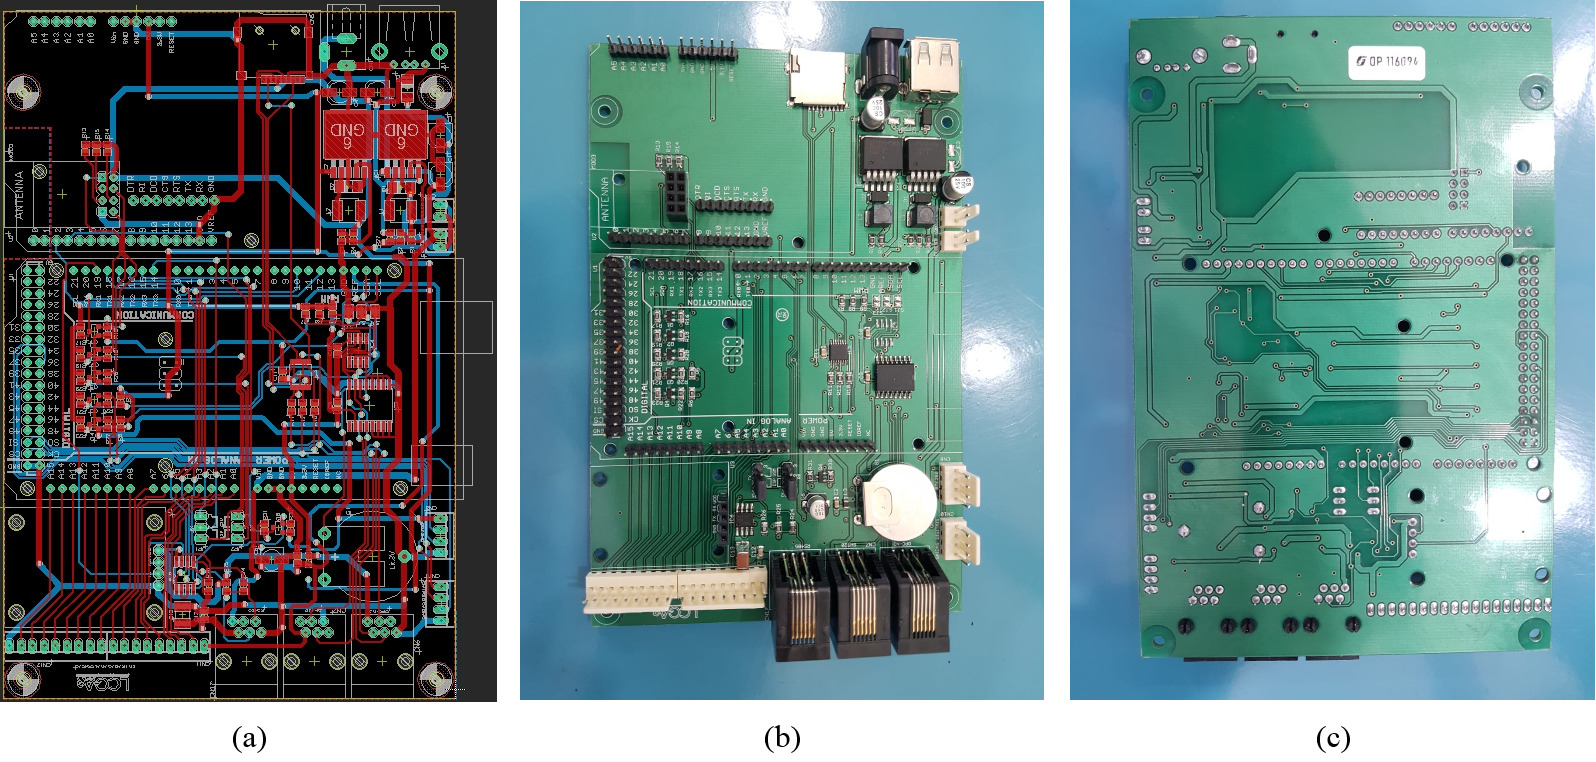
\includegraphics[width=1\linewidth]{chapters//2-CLEAN/Figuras/CLEAN Arduino Mega Board.jpg}
    \label{fig:clean-arduino-mega-board}
\end{figure}

A Tabela \ref{tab:componentes-clean} do apêndice \ref{apendix: clean-arduino-mega-board} mostra os principais componentes de hardware utilizados na placa, que requer uma tensão de alimentação de 12V, 2A através de um conector de alimentação P4. Possui entradas analógicas para 6 placas de sensores Alphasense da série ISB, barramento RS-485 para futuras expansões, três saídas digitais e conectores para alimentação de ventoinhas de 12V e 5V. A placa foi concebida para suportar conexões Wi-Fi e \textit{GPRS} à Internet. Essas conexões não podem ser utilizadas simultaneamente, o que dependerá de cada aplicação. O usuário pode configurar a placa para usar um ou outro e terá que adaptar o firmware do microcontrolador Arduino correspondentemente.

